\section{Semester 1 Work}
\subsection{Explanation of Scripts}
\subsubsection{Solidworks Manipulation Script}
\textbf{Main file}
\newline
The main code of this section of the tool.  It calls other files that are written in Python, packages them as VBA scripts, and then sends them to Solidworks to execute.
\newline
\textbf{SWOPEN}
\begin{figure}[H]
    \centering
    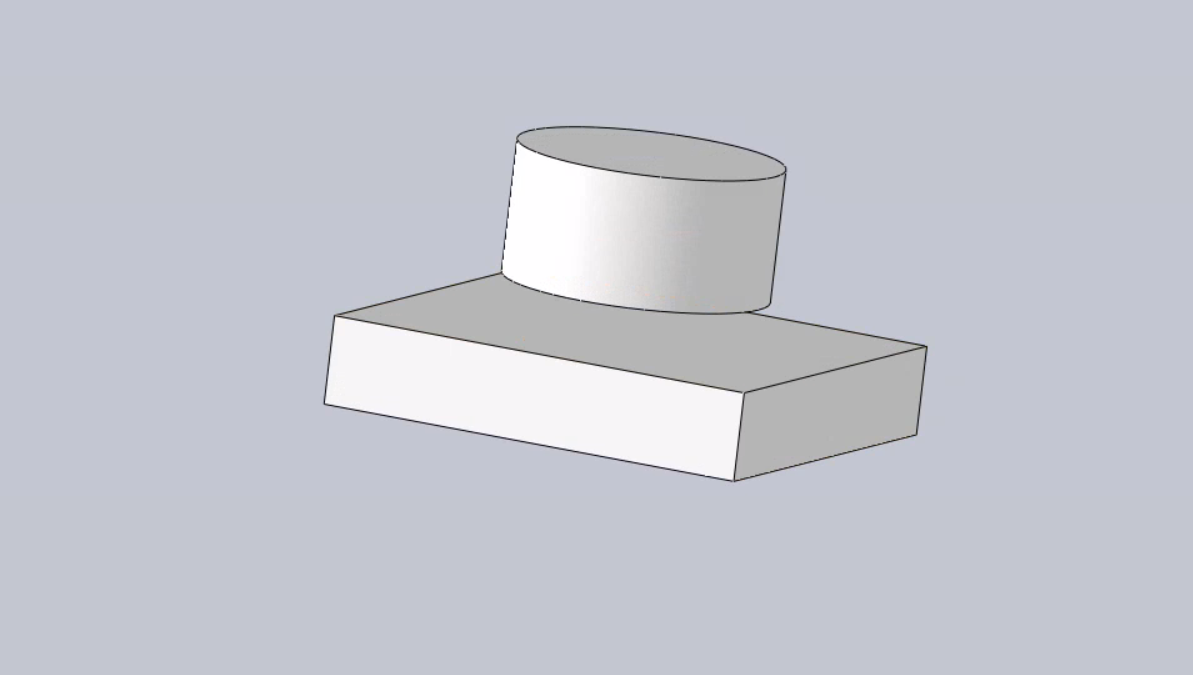
\includegraphics[width=5in]{Figures/Semester 1 Work/Solidworks Open.png}
    \caption{The Solidworks screen when the initial file is opened.}
    \label{fig:SWX Base}
\end{figure}
\indent This code finds the instance of Solidworks installed on the local machine, and opens it.  Then, it opens a step file.  The path of this step file is currently named in the SWOPEN file, but will be moved to be a variable passed from the main file, so it is easily editable by a user.  Figure 8 shows Solidworks just after SWOPEN is run; an unmodified part geometry open.
\newline
\textbf{SWROT}
\newline \indent This code rotates the part in question.  Figure 8 shows Solidworks as it is after SWOPEN runs.  It currently requires the solid body being rotated to be named “part”.  This code finds the running instance of solidworks and attaches to it.  Then, it finds the solid body named “part”.  It inserts a move feature into the feature tree and assigns it to “part” and rotates the part by a set angle.  This angle is passed into the script from main when it is called. Right now, the center of rotation is the origin of the Solidworks document.  This will be changed later on.  
Figure 9 shows the Feature Tree after the rotation feature has been inserted.
\begin{figure}[H]
    \centering
    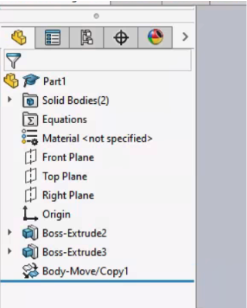
\includegraphics[width=5in]{Figures/Semester 1 Work/Solidworks Feature Tree.png}
    \caption{The feature tree in Solidworks, showing the inserted feature to rotate the part.}
    \label{fig:SWX Tree}
\end{figure}
\begin{figure}[H]
    \centering
    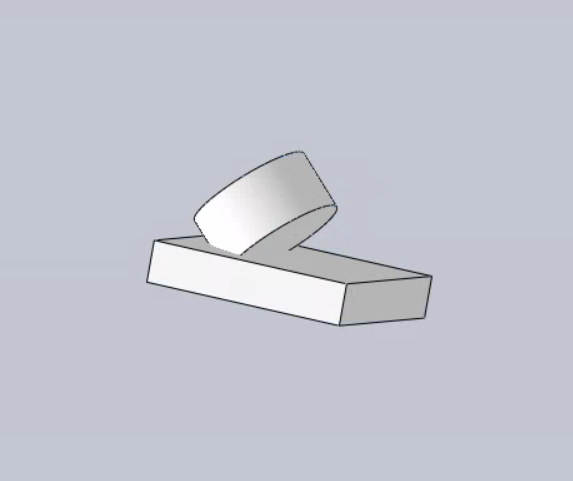
\includegraphics[width=0.5\linewidth]{Figures/Semester 1 Work/Solidworks Rotated.png}
    \caption{The part as rotated by SWROT.  Note the interference.}
    \label{fig:SWX Rotated}
\end{figure}

\indent ANSYS requires the build plate to be located at Z=0, so rotating a part about the origin of the document is not a good idea.  It will cause the part to collide with the build plate.  Future updates to the code will have logic to find the center of gravity of the part being rotated, and rotate it about that, or interference detection along with moving the part until it doesn’t interfere with the build plate.  Figure 10 shows the part that has been rotated, and displays the collision that typically occurs.
\newline \textbf{SWEXPORT}
\newline \indent This script exports the modified document out of Solidworks as a step file.  It takes in the naming convention as an input from main and appends it to the file name when saving the file.  
\subsubsection{ANSYS Execution Script}
\textbf{Main}
\newline \indent The main is responsible for opening the instance of ANSYS mechanical, and calling the following scripts to run the simulation.
\textbf{Call Template}
This script opens the template for LPBF that is included in the folder for the code.  The template needs to exist because the coupled simulation that ANSYS uses for residual stress in LPBF is not available to call from the PYANSYS library.  To get around this limitation and keep the code all in Python, the template was used, and edited with the Python script.  This does lead to a bit of artifacting, but the results are not affected.
Delete Geom
	Because a template was used for this Python script, there is a bit of cleanup that needs to be done.  The template needed to have a geometry and finished simulation inside, so that needs to be removed.  The Delete Geom script deletes the preexisting geometry of the original simulation in the template to make room for the new one.
Import Geom
	This script imports geometry from a step file.  Right now the file is hard coded into the import geom document, but an upcoming improvement is passing the step file from main, which receives it from the Solidworks part manipulation script.  It also assigns the imported bodies to “part” and “base” within the AM simulation process.  This script then deletes the existing mesh controls from the template simulation.
\textbf{Mesh}
\begin{figure}[H]
    \centering
    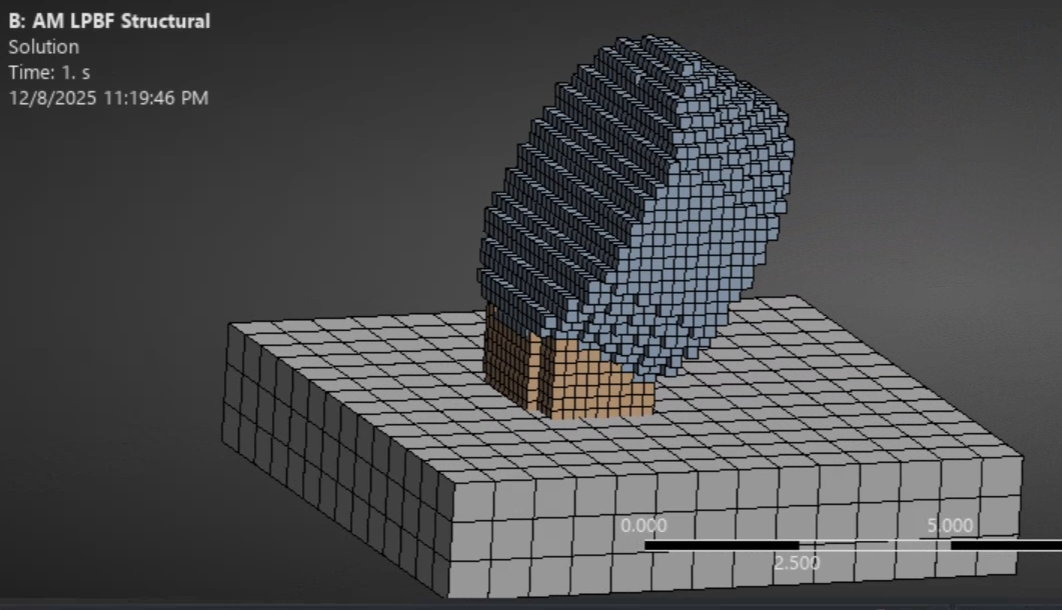
\includegraphics[width=0.5\linewidth]{Figures/Semester 1 Work/Voxel.png}
    \caption{The meshed part; note the voxelized mesh.}
    \label{fig:Voxel}
\end{figure}
\begin{figure}[H]
    \centering
    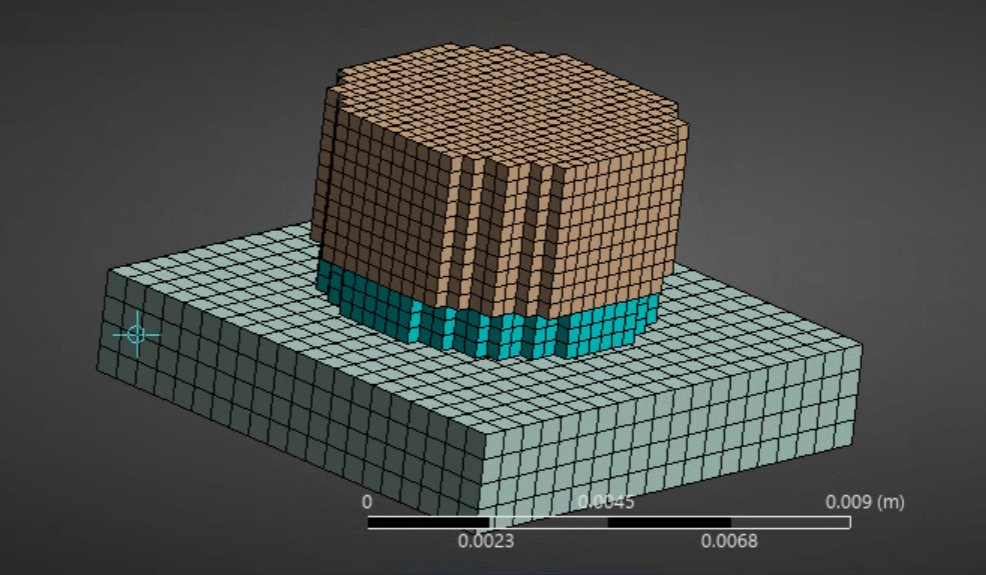
\includegraphics[width=5in]{Figures/Semester 1 Work/Supports.png}
    \caption{The auto-generated supports.}
    \label{fig:Supports}
\end{figure}

This script generates commands ANSYS to generate a mesh for the imported geometry.  It starts off  by defining the global mesh size, then assigns refinements and methods to certain geometries based on the part names.  Then, ANSYS meshes the parts; the meshed setup is shown in Figure 11.  Once this is done, the script deletes the supports that were present for the deleted geometry and defines the parameters for the supports that the new geometry will use.  Figure 12 shows the supports as generated by the script.
Temp and Run
\begin{figure}[H]
    \centering
    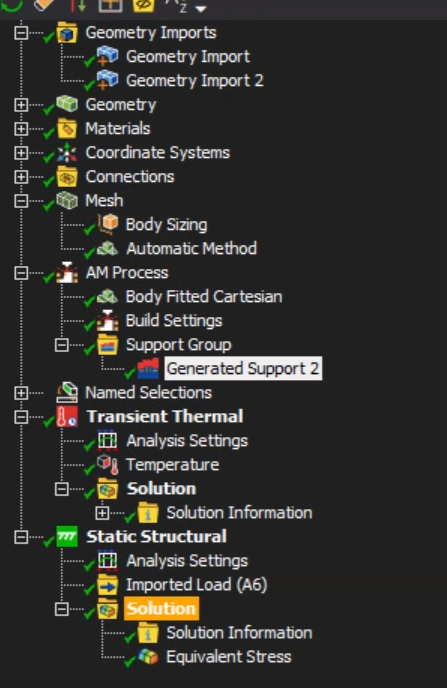
\includegraphics[width=5in]{Figures/Semester 1 Work/ANSYS _Tree.png}
    \caption{The feature tree as modified by the script.}
    \label{fig:ANSYS Tree}
\end{figure}
	Temp and run is the final script in the running of the simulation.  It sets the temperature of the thermal aspect of the simulation, then commands the simulation to solve.  Figure 13 shows the feature tree of the script, including the Temperature and Static Structural that make this a coupled simulation.  Under Geometry Imports, it can be seen that there are two items; this is a result of using the template; the geometry was deleted from the first import, and the geometry from the second was used.
\begin{figure}[H]
    \centering
    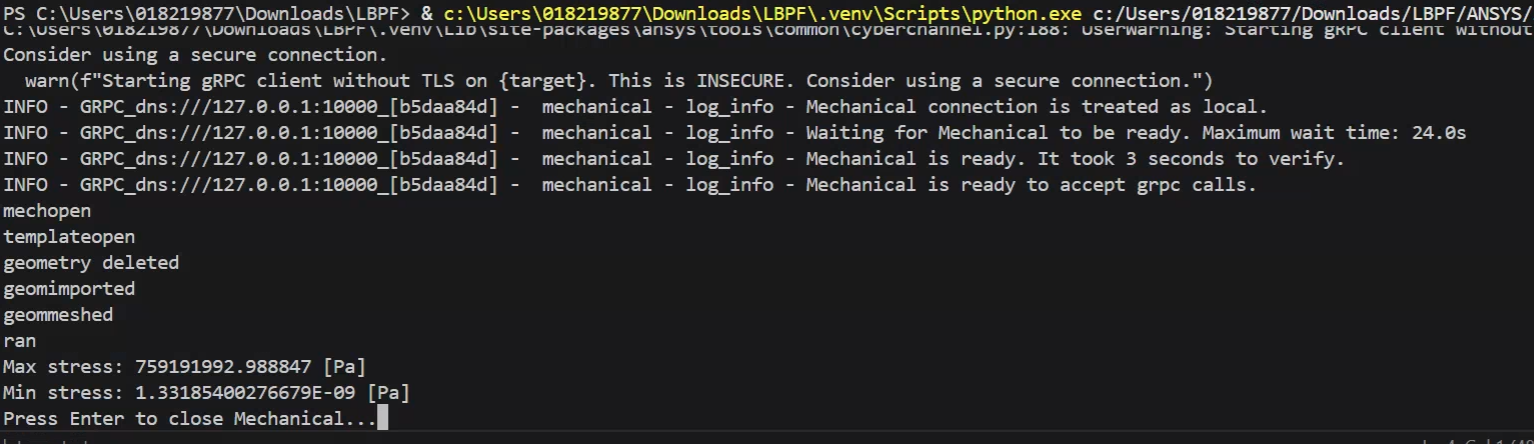
\includegraphics[width=5in]{Figures/Semester 1 Work/Terminal.png}
    \caption{The terminal after the script has run.}
    \label{fig:Terminal}
\end{figure}
Figure 14 shows the terminal as it appears while the ANSYS script is running.  There are checkpoints at which certain strings are printed to let the user know that the script is working correctly.  Currently, the main script receives the stress values from the simulation and shows them.